\documentclass[a4paper,11pt]{extarticle}
\usepackage{geometry}
\usepackage[T1]{fontenc}
\usepackage[utf8]{inputenc}
\usepackage[english,russian]{babel}
\usepackage{amsmath}
\usepackage{amsthm}
\usepackage{amssymb}
\usepackage{fancyhdr}
\usepackage{setspace}
\usepackage{graphicx}
\usepackage{colortbl}
\usepackage{tikz}
\usepackage{pgf}
\usepackage{subcaption}
\usepackage{listings}
\usepackage{indentfirst}
\usepackage[
backend=biber,
style=numeric,
maxbibnames=99
]{biblatex}
\addbibresource{refs.bib}
\usepackage[colorlinks,citecolor=blue,linkcolor=blue,bookmarks=false,hypertexnames=true, urlcolor=blue]{hyperref}
\usepackage{indentfirst}
\usepackage{mathtools}
\usepackage{booktabs}
\usepackage[flushleft]{threeparttable}
\usepackage{tablefootnote}

\usepackage{chngcntr}
\counterwithin{table}{section}
\counterwithin{figure}{section}

\graphicspath{{graphics/}}

\makeatletter
\makeatother

\geometry{left=2.5cm}
\geometry{right=1.0cm}
\geometry{top=2.0cm}
\geometry{bottom=2.0cm}
\setlength{\parindent}{1.25cm}
\renewcommand{\baselinestretch}{1.5}

\lstset{
  basicstyle=\small\ttfamily,
  breaklines=true,
  frame=single,
  tabsize=4,
}

\newcommand{\bibref}[3]{\hyperlink{#1}{#2 (#3)}}
\addto\captionsrussian{\def\refname{Список источников}}

\begin{document}
\input{title_kr}
\newpage
\setcounter{page}{2}

{
	\hypersetup{linkcolor=black}
	\tableofcontents
}

\newpage

\section*{Аннотация}
\addcontentsline{toc}{section}{Аннотация}

В данной работе описывается реализация программной платформы для организации
распределённых добровольных вычислений, написанной на языке программирования
Rust. Разработанная система реализует децентрализованный протокол распределения
задач между участниками одноранговой сети с применением механизмов
репутационного консенсуса и блокчейн-реестра для прозрачного учёта токенового
вознаграждения. Исполнение пользовательских задач выполняется в изолированных
Docker-контейнерах, что обеспечивает безопасность хост-системы и
воспроизводимость окружения. Для взаимодействия пользователя с системой
разработан кроссплатформенный десктопный графический интерфейс, реализованный
на немедленном (immediate-mode) фреймворке egui. Отказоустойчивость сети
обеспечивается за счёт механизма аренды задач с истечением срока: исполнитель,
не отправивший результат вовремя, подвергается штрафу, а задача возвращается в
очередь для повторного назначения. Полученное программное обеспечение
демонстрирует жизнеспособность децентрализованного подхода к организации
добровольных вычислений и может быть использовано научно-исследовательскими
сообществами и образовательными учреждениями для проведения масштабируемых
вычислительных экспериментов.

\section*{Ключевые слова}
\addcontentsline{toc}{section}{Ключевые слова}

Распределённые вычисления, одноранговая сеть, BOINC, Rust, блокчейн,
репутационный консенсус, Docker, изолированное исполнение, immediate-mode GUI,
токеновое вознаграждение.

\pagebreak

\section{Введение}

В современном мире технологии играют важную роль во всех сферах нашей жизни и
деятельности. В связи с этим, одной из актуальных задач является разработка и
усовершенствование различных вычислительных систем, способных облегчить решение
сложных задач и обеспечить эффективное использование вычислительных ресурсов.
Распределённые вычислительные сети представляют собой один из наиболее ярких
примеров таких систем: они объединяют большое количество географически
разнесённых компьютеров в единый вычислительный комплекс, способный решать
задачи, превосходящие по сложности возможности любого отдельно взятого
устройства.

Одним из наиболее известных представителей данного класса систем является
проект BOINC (Berkeley Open Infrastructure for Network Computing)~\cite{boincwebsite},
который применяется для решения научных задач самой разной природы~--- от
расшифровки генома и поиска новых лекарств до моделирования астрофизических
процессов. Идея, на которой построен BOINC, заключается в том, что любой
владелец персонального компьютера может отдать часть своих простаивающих
вычислительных ресурсов в пользу научного проекта и таким образом сделать вклад
в общее дело. За годы существования платформы было реализовано множество
успешных проектов, использующих её инфраструктуру~\cite{anderson_boinc}.

Однако, несмотря на популярность подобных систем, существующие реализации
обладают рядом ограничений. Во-первых, классическая архитектура BOINC основана
на централизованной модели: каждый научный проект разворачивает собственный
сервер, который занимается распределением задач, верификацией результатов и
учётом вкладов волонтёров~\cite{boincwebsite_arcitecture}. Такая модель
накладывает высокие требования на администратора проекта, требует
значительных операционных издержек и создаёт единую точку отказа. Во-вторых,
поскольку каждый проект изолирован, отсутствует общий протокол вознаграждения,
который позволил бы участнику переносить накопленный <<капитал доверия>> между
проектами или направлять заработанные ресурсы на финансирование других задач.

Предлагаемая курсовая работа направлена на разработку альтернативной платформы,
которая устраняет указанные недостатки. Разработанная система построена на
децентрализованной одноранговой архитектуре, использует механизм репутационного
консенсуса для верификации результатов, ведёт учёт вознаграждений с помощью
неизменяемого блокчейн-реестра и выполняет пользовательские задачи в
изолированных Docker-контейнерах, что обеспечивает безопасность и
воспроизводимость. Реализация выполнена на языке программирования
Rust~\cite{rust_book}, что позволяет добиться высокой производительности и
безопасности памяти без накладных расходов на сборку мусора. Целью настоящей
работы является создание прототипа подобной системы и проверка
работоспособности предложенных решений на наборе модульных тестов.

\section{Постановка задачи}

Необходимо разработать программное обеспечение для организации распределённых
добровольных вычислений, способное распределять пользовательские задачи между
участниками одноранговой сети и обеспечивать корректность их выполнения. Система
должна работать без единого центрального сервера: каждый узел сети должен иметь
возможность выступать в роли координатора (публикующего задачи) или исполнителя
(выполняющего задачи) в зависимости от конфигурации. Помимо ядра протокола,
необходимо разработать графический клиент, позволяющий пользователю подключаться
к сети, создавать проекты, публиковать задачи и мониторить состояние сети.

Функциональные требования к разрабатываемой системе формулируются следующим
образом. Прежде всего, координатор должен иметь возможность регистрировать
проекты и пополнять их баланс из собственных средств, после чего публиковать в
рамках проекта пользовательские задачи с указанием размера вознаграждения и
текста скрипта. Каждая задача должна назначаться по очереди нескольким
независимым исполнителям, которые независимо вычисляют результат и отправляют
координатору хэш полученного ответа. Координатор принимает результат как
корректный, если суммарная репутация исполнителей, отправивших одинаковый хэш,
достигает заранее заданного порога кворума. Все финансовые операции~--- как
начальное зачисление токенов, так и выплаты вознаграждения и штрафы за
недобросовестное поведение~--- должны фиксироваться в неизменяемом блокчейн-реестре,
обеспечивающем возможность последующего аудита. Исполнитель, которому назначена
задача, должен подтвердить её выполнение в течение ограниченного интервала
времени (аренды); при нарушении срока он должен подвергаться штрафу, а задача~---
возвращаться в очередь для повторного назначения. Помимо протокольной части,
система должна предоставлять кроссплатформенный графический интерфейс,
позволяющий выполнять перечисленные действия в удобной для пользователя форме.

Нефункциональные требования также носят существенный характер. Реализация должна
быть кроссплатформенной и собираться без модификации исходного кода на
операционных системах семейства macOS, Linux и Windows. Сетевое взаимодействие
между узлами должно осуществляться поверх TCP, а сообщения~--- сериализоваться в
текстовом формате JSON, что упрощает отладку и анализ трафика. Хранилище
блокчейн-реестра должно поддерживать криптографическую проверку целостности,
позволяющую обнаружить любое постфактумное вмешательство в историю транзакций.
Наконец, выполнение пользовательских задач должно происходить в условиях,
исключающих возможность негативного воздействия на устройство исполнителя, что
подразумевает использование некоторой формы изолированного окружения.

\section{Обзор литературы}

Изучение существующих решений началось с работы~\cite{anderson_boinc}, в которой
описана архитектура платформы BOINC и принципы её работы. Из данной публикации
было выявлено, что каждый проект BOINC управляет собственным сервером, который
рассылает задачи волонтёрам с учётом характеристик их оборудования и
предпочтений. Полученная информация позволила сформулировать идею о хранении
метаинформации об участниках сети и о фильтрации задач по их аппаратным
требованиям. Развитие данной идеи приведено в более поздней статье того же
автора~\cite{boinc_article}, где обсуждается глобальное планирование
вычислительных задач и предлагаются модели справедливого распределения нагрузки
между конкурирующими проектами.

Существенную роль в формировании архитектурных требований сыграла
статья~\cite{The_Condor_Experience}, посвящённая опыту разработки распределённой
сети The Condor. Из этой работы были позаимствованы базовые принципы управления
ресурсами участников: право исполнителя в любой момент отказаться от задачи,
необходимость многоуровневой изоляции пользовательского кода и обязательность
механизмов обнаружения сбойных узлов. Авторы The Condor подробно описывают
проблемы, возникающие при выполнении произвольного пользовательского кода на
устройстве исполнителя, и предлагают использовать многоуровневую песочницу для
ограничения доступа задачи к файловой системе и сети.

Вопросы экономического планирования в распределённых средах рассматриваются в
работе~\cite{economic_model_article}, где предлагается модель планирования
потока заданий и справедливого разделения ресурсов в распределённых
вычислительных средах, позволяющая учитывать требования пользователей виртуальной
организации к эффективности и качеству выполнения своих заданий. На основе данной
работы в настоящем проекте была реализована система квот и токенового
вознаграждения, где каждая задача имеет указанную постановщиком стоимость, а
исполнители получают вознаграждение пропорционально вкладу.

Для проектирования механизма репутации использовалась работа~\cite{eigentrust},
в которой описан алгоритм EigenTrust для управления репутацией в одноранговых
сетях. В отличие от полной реализации алгоритма EigenTrust, требующего
итеративного решения задачи о собственном векторе матрицы доверия, в настоящей
работе применяется упрощённая схема: репутация участника представляется
неотрицательным целым числом, увеличивающимся при подтверждении результата и
уменьшающимся при отклонении или истечении аренды. Это решение позволило
сохранить ключевые свойства репутационного механизма при существенной экономии
вычислительных ресурсов.

Теоретическим основанием для разработки механизма консенсуса послужили
классические работы по согласованию в распределённых системах. Прежде всего,
это работа~\cite{byzantine_generals}, в которой сформулирована задача
византийских генералов и доказана невозможность достижения согласия более чем
с одной третью предателей в синхронной сети. Более практически ориентированный
протокол согласования описан в работе~\cite{pbft}, представляющей алгоритм
Practical Byzantine Fault Tolerance. Хотя полное применение PBFT в рамках
курсовой работы не предполагалось, идеи кворумного голосования и весовой суммы
голосов нашли отражение в реализованном механизме консенсуса.

Наконец, для проектирования блокчейн-реестра была изучена основополагающая
работа~\cite{nakamoto_bitcoin}, в которой описана идея неизменяемой цепочки
блоков, связанных через криптографические хэши, а также работа Меркла о
криптографических деревьях~\cite{merkle_1979}. В качестве базовой хэш-функции
для построения цепочки выбрана SHA-256, описанная в стандарте~\cite{fips_180_4}.
Применение изолированных контейнеров для безопасного выполнения произвольного
кода описано в работе~\cite{merkel_docker} и официальной документации
Docker~\cite{docker_docs}.

\section{Анализ существующих решений}

Прежде чем приступить к проектированию собственной системы, были изучены
наиболее значимые существующие платформы для организации распределённых
добровольных вычислений. Целью анализа являлось выявление ключевых ограничений
имеющихся решений и обоснование архитектурных решений, принятых в настоящей
работе.

\textbf{BOINC.} Платформа BOINC~\cite{boincwebsite, anderson_boinc} является
де-факто стандартом в области добровольных вычислений и насчитывает десятки
активных научных проектов. Тем не менее её архитектура основана на строго
централизованной модели: каждый проект разворачивает и администрирует
собственный сервер, который является единственной точкой распределения задач и
верификации результатов. Это создаёт две принципиальные проблемы. Во-первых,
при недоступности сервера весь проект оказывается неработоспособным; во-вторых,
система кредитов BOINC является сугубо внутрипроектной~--- накопленная репутация
не переносится между проектами, и единого финансового реестра не существует.
Кроме того, для публикации нового вычислительного проекта требуется развернуть
собственную серверную инфраструктуру, что значительно повышает порог входа.

\textbf{Folding@home.} Проект Folding@home~\cite{foldinghome} специализируется
на моделировании сворачивания белков и добился значительных научных результатов
благодаря многомиллионному сообществу волонтёров. Однако архитектура проекта
полностью централизована, задачи носят прикладной характер (только
молекулярно-динамическое моделирование), система не поддерживает публикацию
произвольных пользовательских задач, а финансовые стимулы для волонтёров
полностью отсутствуют.

\textbf{Golem Network.} Golem~\cite{golem_whitepaper} является наиболее
близким по идеологии к разработанной системе: это децентрализованная P2P-сеть,
позволяющая арендовать вычислительные ресурсы других участников за
вознаграждение. Тем не менее Golem обладает рядом характеристик, снижающих его
практичность в образовательном и исследовательском контексте. Во-первых,
платёжная система построена поверх публичного блокчейна Ethereum, что
предполагает наличие у каждого участника криптовалютного кошелька, оплату
комиссий за газ и подверженность волатильности курса токена GLM. Во-вторых,
Golem не реализует встроенного механизма консенсуса для верификации результатов:
корректность вычислений остаётся на ответственности постановщика задачи.
В-третьих, инфраструктура проекта значительно сложнее в развёртывании.

\textbf{GridCoin.} GridCoin~\cite{gridcoin} представляет собой попытку ввести
криптовалютное вознаграждение за участие в проектах BOINC посредством
механизма Proof-of-Research. Однако данная система не устраняет централизованный
характер самой BOINC: участник по-прежнему должен подключаться к серверам
отдельных проектов, а GridCoin лишь добавляет финансовый слой поверх
существующей инфраструктуры, унаследовав все её ограничения.

Сводное сравнение перечисленных платформ с разработанной системой приведено
в таблице~\ref{tab:comparison}.

\begin{table}[h!]
\centering
\caption{Сравнение платформ для организации распределённых вычислений}
\label{tab:comparison}
\resizebox{\linewidth}{!}{%
\begin{tabular}{@{}lcccc@{}}
\toprule
\textbf{Критерий} & \textbf{BOINC} & \textbf{Folding@home} & \textbf{Golem} & \textbf{Наша система} \\
\midrule
Архитектура & Централиз. & Централиз. & P2P & P2P \\
Единая точка отказа & Есть & Есть & Нет & Нет \\
Универсальность задач & Ограничена & Нет & Да & Да \\
Изоляция кода & Частичная & Нет & Docker/VM & Docker \\
Верификация результатов & Дублирование & Сервер & Нет & Репут. консенсус \\
Встроенная экономика & Кредиты & Нет & Внешний блокчейн & Встроенный блокчейн \\
Устойчивость к Byzantine & Нет & Нет & Нет & Да \\
Крипто-кошелёк & Не нужен & Не нужен & Обязателен & Не нужен \\
\bottomrule
\end{tabular}%
}
\end{table}

Анализ таблицы позволяет выделить ключевые преимущества разработанной системы
над рассмотренными аналогами. По сравнению с BOINC и Folding@home система
полностью избавлена от централизованного сервера и единой точки отказа: при
выходе любого узла из строя сеть продолжает функционировать, поскольку любой
оставшийся узел может принять роль координатора. Встроенный блокчейн-реестр
обеспечивает сквозную прозрачность всех финансовых операций без зависимости от
внешних платёжных систем, а репутационно-взвешенный консенсус~--- единственный
из рассмотренных механизмов~--- обеспечивает автоматическую верификацию
результатов с устойчивостью к недобросовестным участникам. По сравнению с Golem
система существенно ниже по барьеру входа: не требует криптовалютного кошелька,
не зависит от состояния публичной сети Ethereum и не предполагает никаких
транзакционных комиссий. Наконец, сетевая и ресурсная изоляция Docker-контейнеров
в сочетании с жёсткими ограничениями процессора, памяти и времени выполнения
обеспечивает уровень безопасности хост-системы, отсутствующий у большинства
конкурирующих решений.

\section{Анализ существующих решений}

Прежде чем приступить к проектированию собственной системы, были изучены
наиболее значимые существующие платформы для организации распределённых
добровольных вычислений. Целью анализа являлось выявление ключевых ограничений
имеющихся решений и обоснование архитектурных решений, принятых в настоящей
работе.

\textbf{BOINC.} Платформа BOINC~\cite{boincwebsite, anderson_boinc} является
де-факто стандартом в области добровольных вычислений и насчитывает десятки
активных научных проектов. Тем не менее её архитектура основана на строго
централизованной модели: каждый проект разворачивает и администрирует
собственный сервер, который является единственной точкой распределения задач и
верификации результатов. Это создаёт две принципиальные проблемы. Во-первых,
при недоступности сервера весь проект оказывается неработоспособным; во-вторых,
система кредитов BOINC является сугубо внутрипроектной~--- накопленная репутация
не переносится между проектами, и единого финансового реестра не существует.
Кроме того, для публикации нового вычислительного проекта требуется развернуть
собственную серверную инфраструктуру, что значительно повышает порог входа.

\textbf{Folding@home.} Проект Folding@home~\cite{foldinghome} специализируется
на моделировании сворачивания белков и добился значительных научных результатов
благодаря многомиллионному сообществу волонтёров. Однако архитектура проекта
полностью централизована, задачи носят прикладной характер (только
молекулярно-динамическое моделирование), система не поддерживает публикацию
произвольных пользовательских задач, а финансовые стимулы для волонтёров
полностью отсутствуют.

\textbf{Golem Network.} Golem~\cite{golem_whitepaper} является наиболее
близким по идеологии к разработанной системе: это децентрализованная P2P-сеть,
позволяющая арендовать вычислительные ресурсы других участников за
вознаграждение. Тем не менее Golem обладает рядом характеристик, снижающих его
практичность в образовательном и исследовательском контексте. Во-первых,
платёжная система построена поверх публичного блокчейна Ethereum, что
предполагает наличие у каждого участника криптовалютного кошелька, оплату
комиссий за газ и подверженность волатильности курса токена GLM. Во-вторых,
Golem не реализует встроенного механизма консенсуса для верификации результатов:
корректность вычислений остаётся на ответственности постановщика задачи.
В-третьих, инфраструктура проекта значительно сложнее в развёртывании.

\textbf{GridCoin.} GridCoin~\cite{gridcoin} представляет собой попытку ввести
криптовалютное вознаграждение за участие в проектах BOINC посредством
механизма Proof-of-Research. Однако данная система не устраняет централизованный
характер самой BOINC: участник по-прежнему должен подключаться к серверам
отдельных проектов, а GridCoin лишь добавляет финансовый слой поверх
существующей инфраструктуры, унаследовав все её ограничения.

Сводное сравнение перечисленных платформ с разработанной системой приведено
в таблице~\ref{tab:comparison}.

\begin{table}[h!]
\centering
\caption{Сравнение платформ для организации распределённых вычислений}
\label{tab:comparison}
\resizebox{\linewidth}{!}{%
\begin{tabular}{@{}lcccc@{}}
\toprule
\textbf{Критерий} & \textbf{BOINC} & \textbf{Folding@home} & \textbf{Golem} & \textbf{Наша система} \\
\midrule
Архитектура & Централиз. & Централиз. & P2P & P2P \\
Единая точка отказа & Есть & Есть & Нет & Нет \\
Универсальность задач & Ограничена & Нет & Да & Да \\
Изоляция кода & Частичная & Нет & Docker/VM & Docker \\
Верификация результатов & Дублирование & Сервер & Нет & Репут. консенсус \\
Встроенная экономика & Кредиты & Нет & Внешний блокчейн & Встроенный блокчейн \\
Устойчивость к Byzantine & Нет & Нет & Нет & Да \\
Крипто-кошелёк & Не нужен & Не нужен & Обязателен & Не нужен \\
\bottomrule
\end{tabular}%
}
\end{table}

Анализ таблицы позволяет выделить ключевые преимущества разработанной системы
над рассмотренными аналогами. По сравнению с BOINC и Folding@home система
полностью избавлена от централизованного сервера и единой точки отказа: при
выходе любого узла из строя сеть продолжает функционировать, поскольку любой
оставшийся узел может принять роль координатора. Встроенный блокчейн-реестр
обеспечивает сквозную прозрачность всех финансовых операций без зависимости от
внешних платёжных систем, а репутационно-взвешенный консенсус~--- единственный
из рассмотренных механизмов~--- обеспечивает автоматическую верификацию
результатов с устойчивостью к недобросовестным участникам. По сравнению с Golem
система существенно ниже по барьеру входа: не требует криптовалютного кошелька,
не зависит от состояния публичной сети Ethereum и не предполагает никаких
транзакционных комиссий. Наконец, сетевая и ресурсная изоляция Docker-контейнеров
в сочетании с жёсткими ограничениями процессора, памяти и времени выполнения
обеспечивает уровень безопасности хост-системы, отсутствующий у большинства
конкурирующих решений.

\pagebreak

\section{Выбор инструментов разработки}

К выбору инструментов разработки было решено подойти ответственно, поскольку
он во многом определяет надёжность и производительность итогового продукта. В
качестве основного языка программирования был выбран Rust~\cite{rust_book}~---
системный компилируемый язык, ориентированный на разработку
высокопроизводительных систем с гарантиями безопасности памяти. Этот выбор
обосновывается несколькими соображениями. Прежде всего, гарантии безопасности
памяти, обеспечиваемые системой владения и проверкой заимствований на этапе
компиляции, позволяют избежать целого класса ошибок, характерных для языков с
ручным управлением памятью, без накладных расходов на сборщик мусора, типичных
для языков высокого уровня. Помимо этого, экосистема Rust содержит хорошо
проработанные библиотеки для асинхронного программирования, криптографии,
работы с сетью и графическим интерфейсом, что позволило реализовать все
необходимые компоненты системы без привлечения сторонних программ на других
языках.

Для организации конкурентного выполнения сетевых операций был использован
асинхронный рантайм Tokio~\cite{tokio_rs}~--- наиболее распространённое в
экосистеме Rust решение для построения сетевых сервисов. Tokio предоставляет
эффективный планировщик задач, способный обслуживать большое количество
одновременных соединений на ограниченном числе системных потоков, а также
богатый набор примитивов синхронизации, таких как многопроизводительные каналы
MPSC, широковещательные каналы и асинхронные мьютексы. Использование Tokio
позволило построить сетевой слой системы по событийной модели, в которой каждое
входящее соединение обслуживается независимой задачей, а обмен сообщениями
между задачами и графическим интерфейсом происходит через каналы.

Для разработки графического интерфейса была выбрана библиотека
egui~\cite{egui_crate}, реализующая немедленный (immediate-mode) подход к
построению GUI: интерфейс не описывается как иерархия объектов-виджетов, а
перерисовывается полностью на каждом кадре исходя из текущего состояния
программы. Такой подход избавляет разработчика от необходимости синхронизации
состояния модели и виджетов и существенно упрощает реализацию динамических
интерфейсов с часто изменяющимися данными. Поскольку библиотека написана на
чистом Rust и не зависит от системных GUI-фреймворков, оконная оболочка eframe
позволяет собирать одно и то же приложение под macOS, Linux и Windows без
модификации исходного кода.

В качестве хэш-функции для построения блокчейн-реестра был выбран алгоритм
SHA-256, описанный в стандарте~\cite{fips_180_4} и реализованный в крейте sha2
из набора RustCrypto. Выбор именно SHA-256, а не более современных функций
семейства SHA-3 или BLAKE3, обусловлен повсеместной распространённостью данного
алгоритма, его хорошо изученными криптографическими свойствами и широкой
поддержкой в стандартных библиотеках различных языков, что облегчает возможную
интероперабельность с другими реализациями.

Для изолированного выполнения пользовательских задач была применена
контейнеризация Docker~\cite{merkel_docker, docker_docs}. Взаимодействие с
демоном Docker осуществляется через крейт bollard, предоставляющий нативный
Rust-клиент к Docker Engine API. Docker был выбран по нескольким причинам:
он обеспечивает достаточный уровень изоляции для задачи запуска
непроверенного кода, поддерживается на всех целевых платформах, имеет
устоявшийся протокол распространения образов и широко распространён среди
разработчиков, что снижает порог входа для конечных пользователей системы.

\section{Архитектура системы}

Архитектура разработанной системы основана на одноранговой (peer-to-peer)
модели, в которой отсутствует единый центральный сервер, а каждый узел сети
может выступать в одной из двух ролей. Узел в роли координатора принимает
входящие TCP-соединения от других участников, хранит состояние сети~--- список
участников, проекты, задачи, блокчейн-реестр~--- и осуществляет распределение
задач между подключёнными исполнителями. Узел в роли исполнителя, напротив,
подключается к координатору, периодически запрашивает у него новые задачи,
выполняет их и отправляет результаты. В рамках одного процесса допускается
одновременная работа нескольких логических узлов, что особенно удобно для
проведения локального тестирования: один и тот же бинарный файл может быть
запущен как координатор, а на других машинах~--- как исполнители, либо все
роли могут быть смоделированы в пределах одного процесса.

Внутренняя организация приложения построена на разделении ответственности
между двумя параллельными контекстами исполнения. Главный поток операционной
системы занят циклом событий графического интерфейса: библиотека eframe
требует, чтобы все вызовы egui производились из основного потока, поскольку
многие графические API ведут себя корректно только в таком режиме. Параллельно
с главным потоком работает пул потоков асинхронного рантайма Tokio, на котором
запущен сетевой актор~--- центральный компонент, реализующий протокол
взаимодействия и хранящий состояние сети. Между графическим интерфейсом и
сетевым актором установлена пара каналов MPSC: командный канал, по которому
GUI отправляет в сетевой слой запросы пользователя (создать проект, опубликовать
задачу, подключиться к узлу), и канал событий, по которому сетевой слой
сообщает в GUI об изменениях состояния (поступление новой задачи, изменение
баланса, обновление списка участников). Использование каналов позволяет
полностью развязать графический интерфейс и сетевую логику: GUI остаётся
отзывчивым даже при длительных сетевых операциях, а сетевой слой может
работать независимо от наличия активного интерфейса.

Сетевой актор внутри себя мультиплексирует два режима работы. В режиме
координатора актор открывает прослушивающий TCP-сокет, ожидает подключений и
для каждого нового соединения запускает отдельную асинхронную задачу,
обрабатывающую входящие сообщения. В режиме исполнителя актор поддерживает
одно исходящее соединение с координатором, периодически запрашивает новые
задачи и обрабатывает входящие сообщения от координатора. Для согласованного
изменения общего состояния между обработчиками соединений используется
широковещательный канал, по которому рассылаются обновления состояния всем
заинтересованным сторонам. Сериализация сообщений выполняется в формате JSON,
а разделение потока данных на отдельные сообщения~--- с использованием
кодека LinesCodec из библиотеки tokio-util, что обеспечивает простоту отладки
и совместимость с инструментами анализа сетевого трафика.

\begin{figure}[h!]
    \centering
    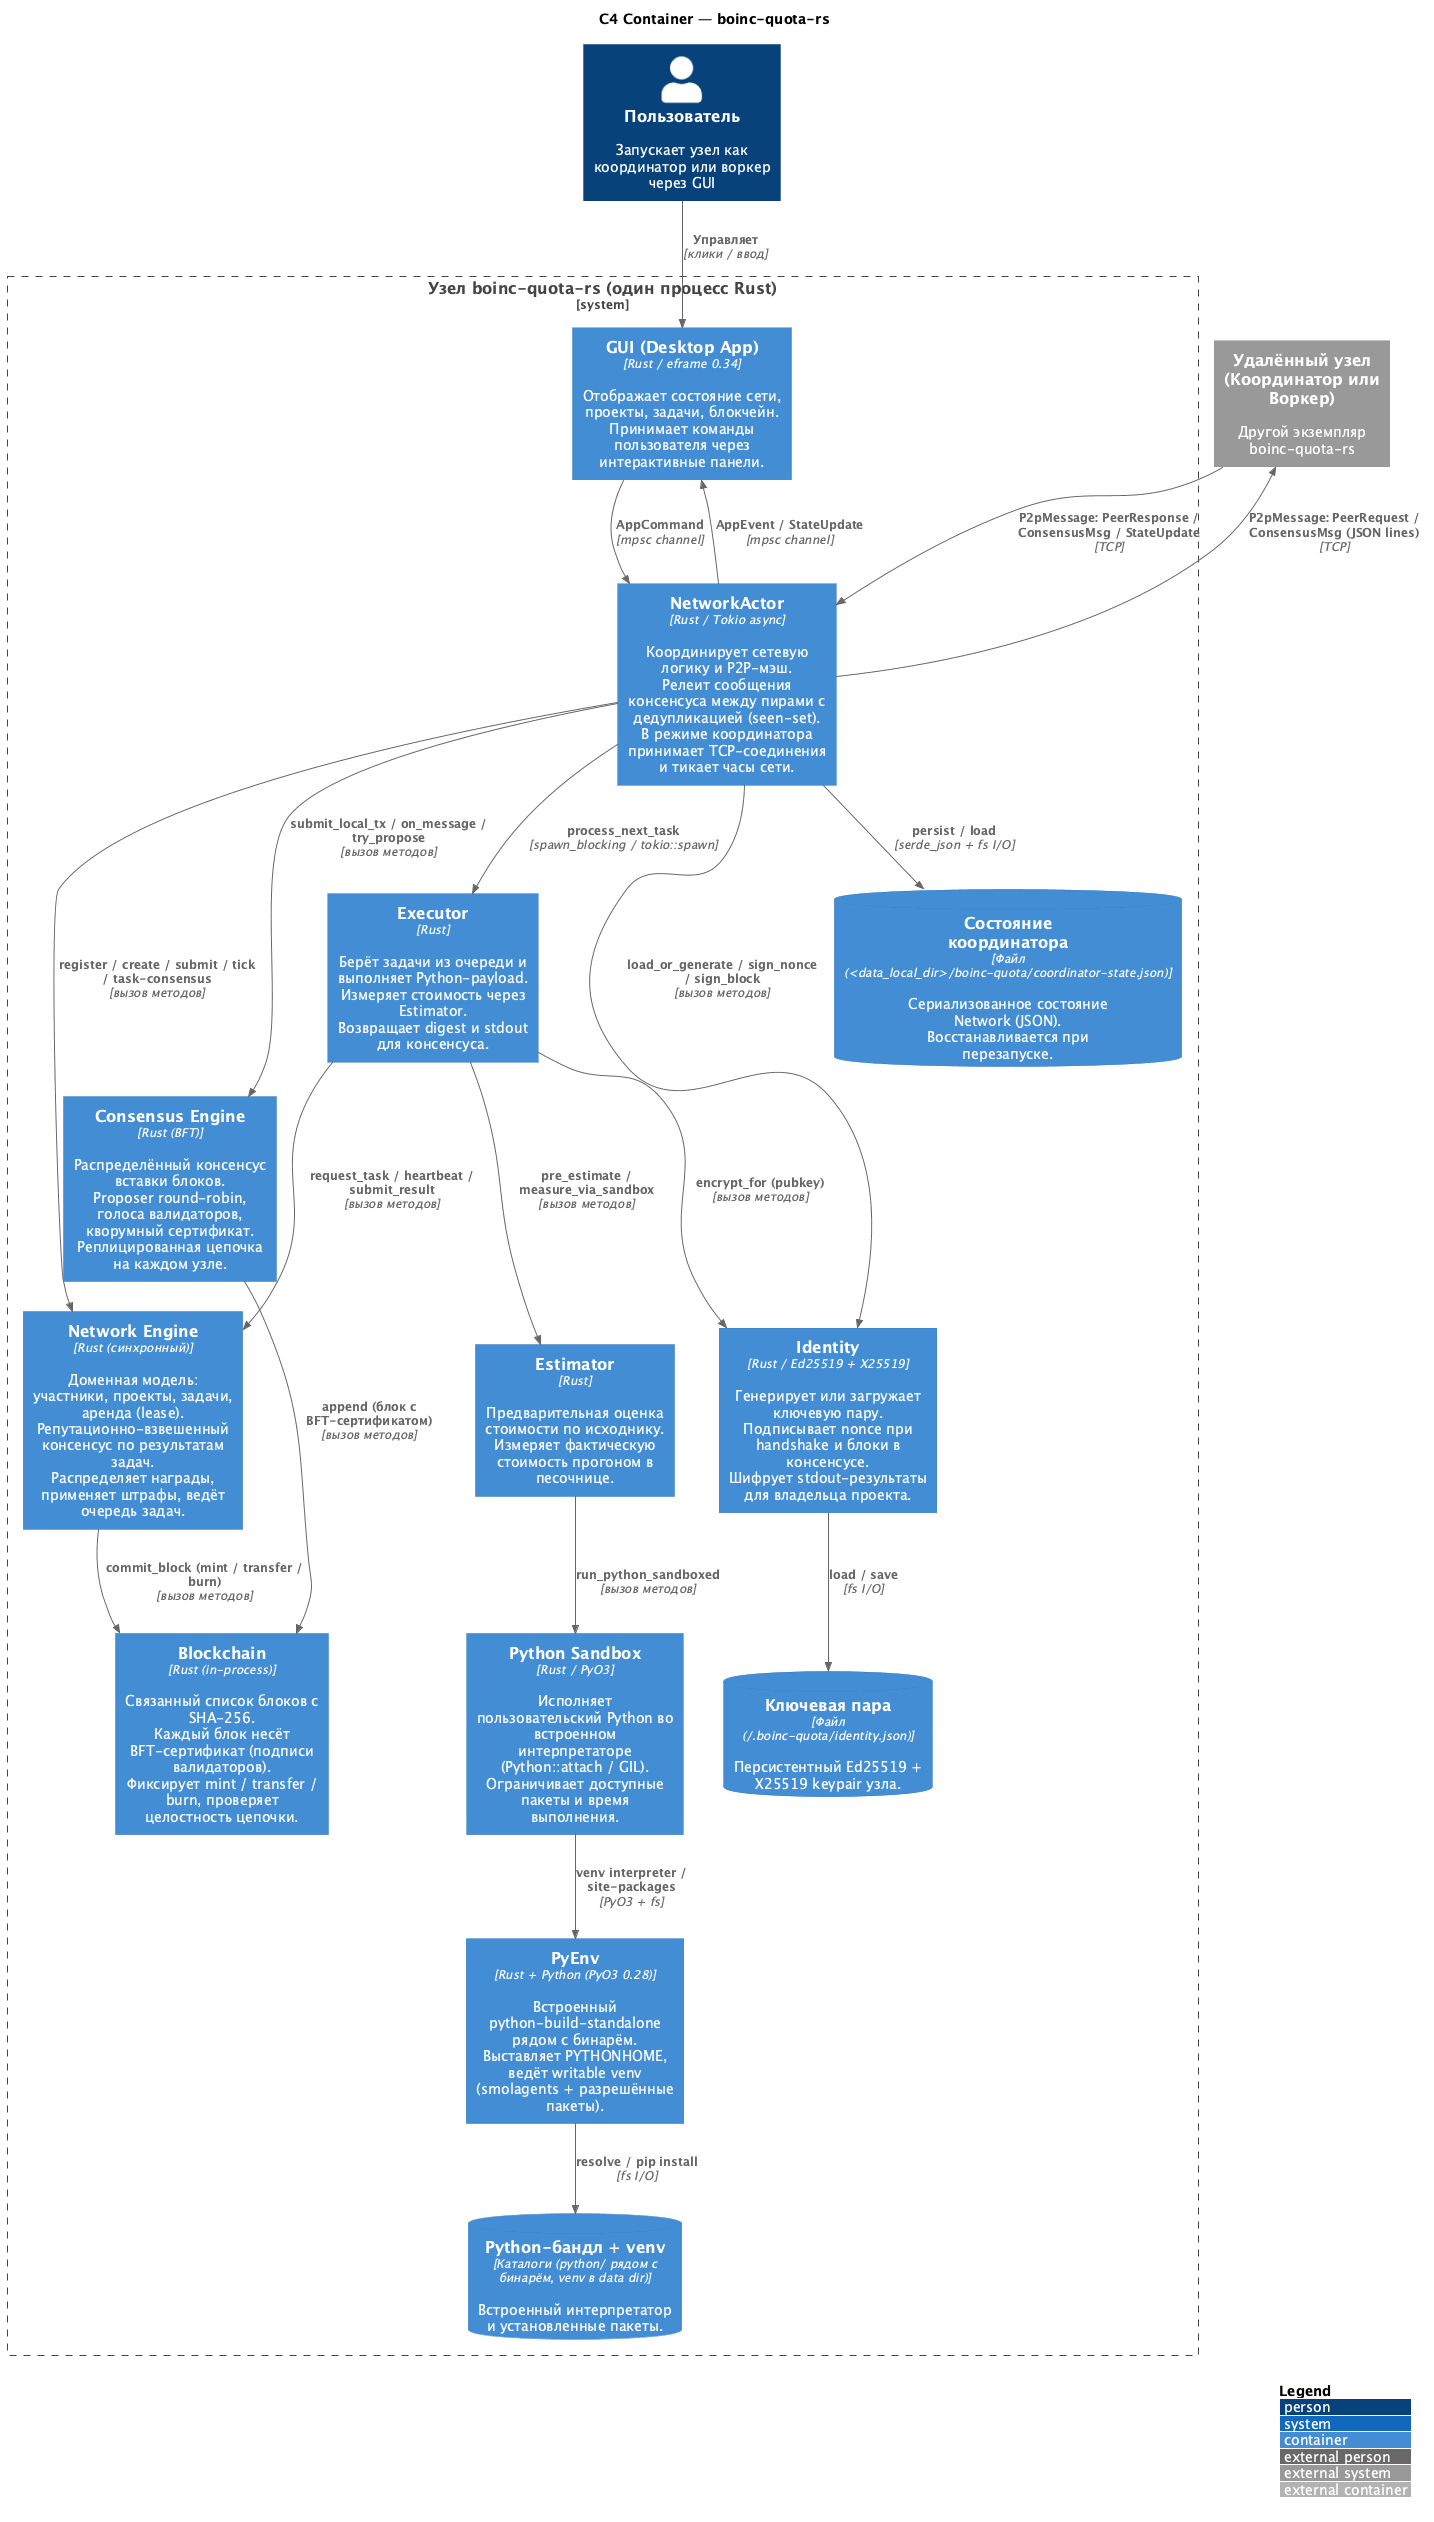
\includegraphics[width=\textwidth]{C4_Container_BOINC_Quota.png}
    \caption{C4-диаграмма контейнеров: компоненты узла и их взаимодействие}
    \label{fig:c4container}
\end{figure}

Поскольку подобная одноранговая архитектура в существенной мере отличается от
классической клиент-серверной модели, применяемой в большинстве реализаций
распределённых сетей, она потребовала проработки ряда нетривиальных вопросов,
связанных с согласованием состояния между узлами и обнаружением выхода из
строя отдельных участников. Эти вопросы рассматриваются в следующем разделе.

\section{Протокол распределённых вычислений}

Центральной частью разработанной системы является протокол распределения и
верификации задач, реализованный в модуле network. Жизненный цикл каждой
задачи описывается конечным автоматом с четырьмя основными состояниями. После
публикации задача оказывается в состоянии <<ожидает назначения>> (Pending) и
помещается в очередь координатора. В этот момент сумма вознаграждения,
указанная постановщиком, резервируется на проектном счёте: квота
\texttt{quota\_available} проекта уменьшается, а \texttt{quota\_locked}
соответственно увеличивается, что фиксируется в блокчейн-реестре как
транзакция Transfer с проектного счёта на временный резерв задачи. Когда
свободный исполнитель запрашивает задачу, координатор выбирает её из очереди
по приоритету: проекты с большим объёмом неосвоенной квоты получают
преимущество, а внутри проекта~--- задачи с большим идентификатором, что
обеспечивает приблизительную справедливость FIFO. Дополнительное условие
выбора~--- исполнитель ранее не присылал отчёт по этой же задаче, чтобы
избежать ситуации, в которой одна и та же сторона голосует за результат
несколько раз. После выбора задачи она переходит в состояние Assigned, и
исполнителю выдаётся аренда сроком \texttt{lease\_timeout\_ticks} тиков. Тик
является дискретной единицей логического времени симуляции: счётчик тиков
продвигается явными вызовами \texttt{network.tick(n)} и не привязан к
астрономическому времени. Такой подход позволяет тестировать временные
инварианты~--- истечение аренды, частоту heartbeat-сообщений~--- детерминированно
и без использования системных таймеров.

Когда исполнитель завершает вычисления, он отправляет координатору отчёт о
выполнении, содержащий хэш результата (digest), идентификатор задачи и
измеренные параметры потребления ресурсов. Координатор регистрирует отчёт и
проверяет, не достигнут ли консенсус по одному из присланных хэшей. Механизм
консенсуса является репутационно-взвешенным: каждый отчёт вносит в общую
сумму голосов вес, равный текущей репутации соответствующего исполнителя,
после чего проверяется, превысила ли суммарная репутация для какого-либо
хэша заданный порог кворума (по умолчанию~--- 2). Если порог достигнут, задача
переходит в состояние Completed: согласившимся исполнителям начисляется
вознаграждение, их репутация увеличивается, а несогласные с консенсусом
исполнители получают штраф. Если же ни один хэш не набрал кворума, но
количество отчётов уже превысило заданный лимит попыток, задача переходит в
состояние Rejected, а зарезервированная сумма возвращается на проектный счёт.

Отдельного внимания заслуживает механизм аренды, обеспечивающий
отказоустойчивость системы. После назначения задачи исполнителю запускается
таймер: если в течение \texttt{lease\_timeout\_ticks} тиков от него не было
получено ни одного отчёта или сообщения о продлении аренды (heartbeat),
координатор считает аренду истёкшей. Истечение аренды интерпретируется как
факт недобросовестного поведения или сбоя у исполнителя: его репутация
уменьшается, с его балансовой записи списывается штраф в виде транзакции Burn,
а сама задача возвращается в очередь Pending для повторного назначения. Такой
механизм позволяет системе автоматически восстанавливаться после сбоев
исполнителей, не требуя явного вмешательства администратора.

Для тестирования устойчивости системы к недобросовестным участникам в
исполнителе реализован режим симуляции византийского поведения. При настройке
параметра надёжности менее 100\% исполнитель с заданной вероятностью отправляет
заведомо искажённый хэш результата, что моделирует ситуацию преднамеренного
саботажа со стороны участника. Поведение исполнителя при этом остаётся
детерминированным и воспроизводимым при фиксированном начальном числе псевдослучайности, что облегчает
воспроизведение тестовых сценариев. Подобный режим позволяет на практике
убедиться в том, что репутационный механизм консенсуса корректно отсекает
влияние недобросовестных голосов и в долгосрочной перспективе приводит к
снижению их репутации до нуля, после чего их голоса перестают учитываться при
кворумном голосовании. Идейно описанный подход к голосованию опирается на
классические работы по византийской устойчивости~\cite{byzantine_generals,pbft}.

Полная последовательность взаимодействий между участниками сети за время
жизни одной задачи~--- от аутентификации исполнителя и публикации задачи до
достижения консенсуса и начисления вознаграждения~--- приведена на рисунке~\ref{fig:sequence}.

\begin{figure}[p]
    \centering
    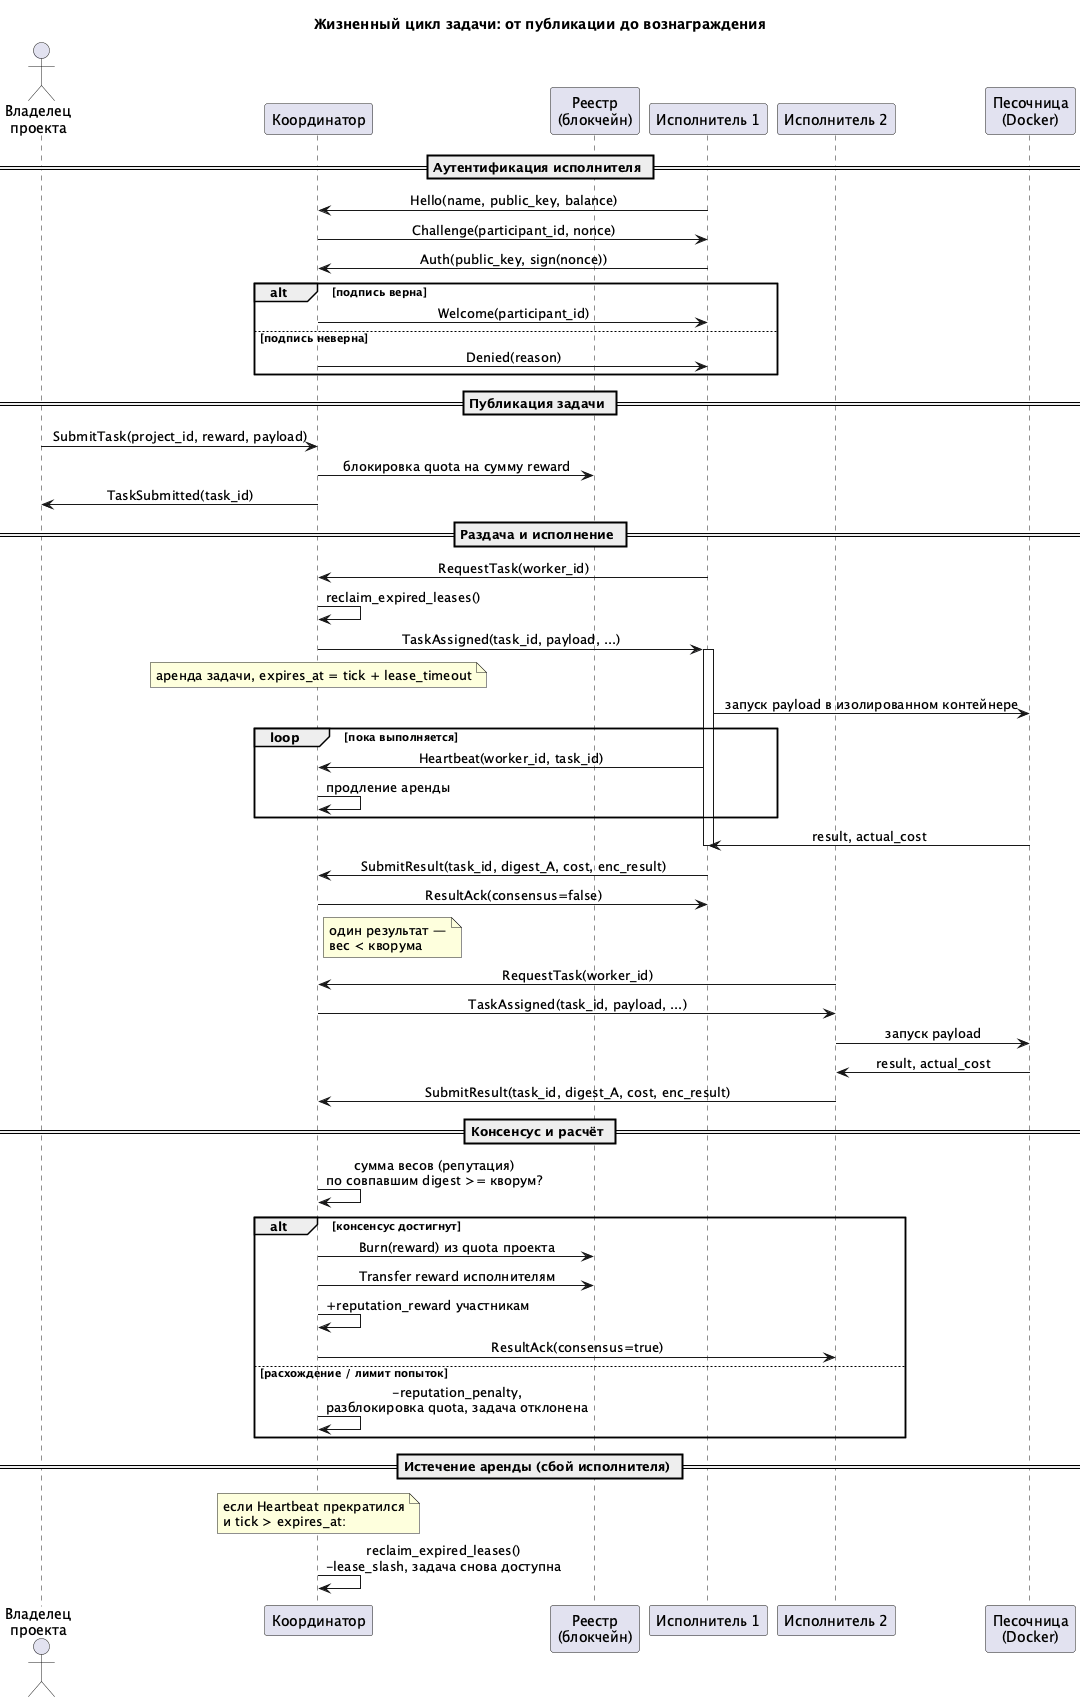
\includegraphics[width=\textwidth,height=0.9\textheight,keepaspectratio]{sequence_task.png}
    \caption{Диаграмма последовательности жизненного цикла задачи}
    \label{fig:sequence}
\end{figure}

\section{Блокчейн-реестр}

Для прозрачного и проверяемого учёта всех финансовых операций в системе
реализован блокчейн-реестр, представляющий собой неизменяемую цепочку блоков,
связанных через криптографические хэши. Идея подобной структуры данных была
предложена ещё в работах по криптографическим деревьям~\cite{merkle_1979} и
получила широкую известность благодаря применению в системе
Bitcoin~\cite{nakamoto_bitcoin}. В рамках настоящего проекта применяется
упрощённая модель блокчейна без распределённого согласования: реестр
поддерживается на стороне координатора и реплицируется на исполнителей
исключительно для целей аудита, что соответствует выбранной архитектуре с
выраженной ролью координатора.

Каждый блок реестра содержит порядковый номер (высоту блока), полезную нагрузку
в виде описания одной транзакции и хэш SHA-256 от заголовка предыдущего блока.
Хэш предыдущего блока вычисляется по конкатенации его номера, сериализованного
представления транзакции и его собственного предшествующего хэша, что
обеспечивает рекурсивную связность всей цепочки. Любая попытка изменить
содержимое исторического блока приводит к изменению его хэша, что в свою
очередь инвалидирует хэш-связку со следующим блоком, и так до конца цепочки.
Таким образом, для подделки одной исторической записи злоумышленнику
потребовалось бы пересчитать хэши всех последующих блоков, что и используется
в качестве свойства неизменяемости. Для криптографической части реестра
применяется алгоритм SHA-256, описанный в стандарте~\cite{fips_180_4}, как
наиболее распространённый и хорошо изученный.

В реестре поддерживаются три типа транзакций. Транзакция Mint описывает
начальное зачисление токенов вновь зарегистрированному участнику и применяется
один раз при создании учётной записи. Транзакция Transfer описывает перевод
токенов между двумя адресами и используется как для финансирования проектов
постановщиками, так и для выплаты вознаграждения исполнителям после успешного
завершения задачи. Транзакция Burn описывает уничтожение токенов и применяется
в качестве меры наказания за истечение аренды или отправку результата, не
совпадающего с консенсусом. Для разделения адресных пространств участников и
проектов проектные счета имеют отдельные адреса, формируемые добавлением
константного смещения $10^9$ к идентификатору проекта, что исключает коллизии
с адресами участников при разумных размерах сети.

Верификация целостности реестра выполняется методом, который последовательно
проходит все блоки и для каждого вычисляет ожидаемый хэш на основе хранимого
содержимого, сравнивая его с фактическим хэшем-связкой следующего блока. При
обнаружении любого несоответствия возвращается ошибка с указанием индекса
повреждённого блока, что позволяет точно локализовать место постфактумного
вмешательства. Данная процедура запускается при каждом запросе баланса, что
гарантирует, что итоговые суммы вычисляются по проверенной истории. Текущий
баланс конкретного адреса определяется как алгебраическая сумма всех
транзакций, в которых данный адрес участвовал в качестве отправителя или
получателя, что соответствует модели <<полного состояния>>, а не модели
непотраченных выходов (UTXO), используемой в Bitcoin.

\section{Исполнитель задач}

Компонент executor отвечает за непосредственное выполнение задач, назначенных
исполнителю координатором. Задача представляет собой полезную нагрузку,
содержащую текст пользовательского Python-кода и набор параметров запуска.
Выбор вычислительного бэкенда происходит автоматически при инициализации
исполнителя в зависимости от доступности Docker-демона в системе. Реализованы
два режима исполнения: основной режим на базе Docker-контейнеров и резервный
режим на базе встроенной изолированной среды CPython.

\textbf{Режим Docker.}
При наличии доступного Docker-демона код задачи выполняется в изолированном
контейнере на основе образа \texttt{python:3.11-alpine}. Взаимодействие с
демоном реализовано через крейт bollard, предоставляющий нативный
асинхронный Rust-клиент к Docker Engine API. Перед запуском контейнера
исполнитель формирует временный каталог с входными файлами и исполняемым
скриптом, после чего монтирует его в контейнер. К параметрам запуска
применяются жёсткие ограничения ресурсов: квота процессорного времени
ограничивается 512 долями (приблизительно половина ядра), доступная память~---
256~МБ, а полное время работы контейнера~--- десятью секундами. Контейнер
запускается в режиме сетевой изоляции (\texttt{network\_mode: none}), что
исключает любые обращения к сети хоста или внешним ресурсам и тем самым
предотвращает целые классы атак, связанных с эксфильтрацией данных.

\textbf{Режим встроенной изолированной среды.}
Если Docker-демон недоступен или в процессе работы возникает ошибка контейнера,
исполнитель автоматически переключается на резервный режим, основанный на
встроенном интерпретаторе CPython. Код задачи выполняется непосредственно
в адресном пространстве процесса через привязки PyO3, однако в строго
ограниченной среде: список допустимых модулей ограничен явным белым списком,
все операции с файловой системой и сетью запрещены на уровне перехвата
встроенных функций, вывод \texttt{print} перенаправляется в буфер памяти
и не достигает консоли хоста. Выполнение ограничивается тем же таймаутом,
что и в Docker-режиме, а по его истечении поток принудительно прерывается.
Данный режим не требует наличия каких-либо внешних зависимостей, что делает
его пригодным как для развёртывания без Docker, так и для модульного
тестирования сетевого протокола и механизма консенсуса.

Параллельно с непосредственным исполнением задачи компонент estimator
выполняет измерение фактического потребления ресурсов: процессорного времени,
максимально занимаемой памяти и реального времени выполнения. Измерения
производятся через системный вызов \texttt{getrusage}, доступный через крейт
libc, и записываются в отчёт о выполнении задачи. Полученные значения
прикрепляются к отчёту, отправляемому координатору, и в дальнейшем могут
использоваться как для аудита, так и для уточнения экономической модели
вознаграждения, например, для дифференцированной выплаты в зависимости от
фактически затраченных ресурсов.

\section{Графический интерфейс}

Графический интерфейс приложения реализован на библиотеке egui~\cite{egui_crate}
в немедленном (immediate-mode) режиме, при котором всё состояние интерфейса
полностью перерисовывается на каждом кадре исходя из текущей модели данных.
Оконная оболочка eframe предоставляет нативное окно операционной системы
размером 960 на 640 пикселей и реализует цикл событий, в котором происходит
сначала обработка входящих событий ввода, а затем перерисовка интерфейса.
Подобный подход к построению GUI существенно упрощает синхронизацию состояния:
при изменении модели нет необходимости явно обновлять виджеты, поскольку на
следующем кадре они будут построены заново исходя из новых данных. Это особенно
полезно для приложений с часто изменяющимся состоянием, к которым относится
монитор распределённой сети.

Интерфейс приложения разделён на пять вкладок, каждая из которых соответствует
одной из основных задач пользователя. Вкладка Connect отвечает за установление
соединения с сетью: в ней пользователь выбирает режим работы узла (координатор
или исполнитель) и указывает адрес для прослушивания или подключения, после
чего сетевой актор инициирует соответствующую операцию через командный канал.
Вкладка Projects отображает список проектов сети с указанием названия, общего
баланса и доступной квоты; координатор может создавать в ней новые проекты и
пополнять их балансы. Вкладка Tasks позволяет публиковать новые задачи с
указанием текста скрипта, размера вознаграждения и принадлежности к проекту,
а также мониторить текущий статус существующих задач с разбивкой по
состояниям. Вкладка Executor содержит настройки исполнителя: максимальное
количество одновременно выполняемых задач, интервал отправки heartbeat-сообщений
и уровень надёжности для симуляции византийского поведения. Наконец, вкладка
Network отображает текущий список участников сети с их репутацией и
балансом, а также журнал транзакций блокчейн-реестра в удобной для чтения
табличной форме.

% TODO: вставить скриншоты вкладок Connect, Projects, Tasks, Network
% \begin{figure}[h!]
%     \centering
%     \includegraphics[width=\textwidth]{tabs_overview.png}
%     \caption{Общий вид графического интерфейса приложения}
%     \label{fig:gui}
% \end{figure}

Обновление состояния интерфейса происходит через канал событий, по которому
сетевой актор присылает уведомления об изменениях. Получив такое событие,
главный поток приложения вызывает методы egui-контекста для запроса
перерисовки, в результате чего обновлённые данные отображаются на следующем
кадре. Поскольку перерисовка происходит только при наличии входящих событий
или ввода пользователя, в спокойном состоянии приложение практически не
потребляет процессорное время, что делает его пригодным для длительной работы
в фоновом режиме на устройстве пользователя.

\section{Тестирование}

Корректность реализации проверяется набором модульных тестов, расположенных
непосредственно в исходных файлах в соответствии с принятыми в экосистеме Rust
соглашениями. Общее количество тестов составляет тридцать шесть, и они
покрывают все основные слои системы: блокчейн-реестр, сетевой протокол,
исполнитель задач и оценщик ресурсов. Запуск всего набора производится
стандартной командой \texttt{cargo test} и не требует наличия внешних
зависимостей вроде запущенного Docker-демона, поскольку тесты используют
режим Mock для исполнения задач и не обращаются к реальной сети.

Двенадцать тестов посвящены проверке блокчейн-реестра. В них проверяется
корректность операций Mint, Transfer и Burn, точность вычисления баланса по
истории транзакций, согласованность пересечений между адресными пространствами
участников и проектов, а также~--- что особенно важно для гарантий неизменяемости~---
обнаружение постфактумных подмен в исторических блоках. Один из ключевых
тестов специально модифицирует поле суммы в произвольном историческом блоке и
убеждается в том, что метод верификации немедленно сообщает об ошибке с
указанием на номер этого блока. Подобная проверка демонстрирует, что выбранная
конструкция хэш-цепочки выполняет своё назначение и обеспечивает заявленный
уровень целостности данных.

Шестнадцать тестов посвящены сетевому протоколу. В них моделируется полный
жизненный цикл задачи от публикации до завершения с применением мок-исполнителей,
имитирующих различные сценарии поведения: совпадение результатов и достижение
консенсуса, отказ части участников, истечение аренды у одного из них,
расхождение результатов и отсутствие консенсуса в пределах лимита попыток, а
также отклонение задачи по достижении этого лимита. Отдельная группа тестов
проверяет корректность пересчёта репутации и баланса участников после каждого
из перечисленных сценариев, что позволяет убедиться в согласованности
протокольной части с блокчейн-реестром.

Три теста посвящены поведению исполнителя в различных условиях: успешное
выполнение задачи и получение вознаграждения, истечение аренды и связанные с
этим штрафы, отсутствие доступных задач и ожидание в состоянии покоя.
Наконец, пять тестов покрывают модуль estimator: они проверяют корректность
предварительной оценки стоимости задачи на основе её описания, фактического
вычисления стоимости после её выполнения и детерминированности измерений.
Прохождение всего набора тестов на момент написания работы подтверждает
работоспособность ключевых компонентов системы и служит дополнительным
основанием для дальнейшего развития проекта.

\section{Заключение}

В результате выполнения курсовой работы было реализовано программное
обеспечение для организации распределённых добровольных вычислений с
децентрализованной одноранговой архитектурой, написанное на языке
программирования Rust. Разработанная система устраняет ряд ограничений,
характерных для классических реализаций подобных платформ, основанных на
централизованной клиент-серверной модели, и демонстрирует жизнеспособность
альтернативного подхода. В частности, реализован протокол распределения и
верификации задач, использующий репутационно-взвешенный консенсус для
устойчивости к недобросовестным участникам, а также механизм аренды задач с
истечением срока для автоматического восстановления после сбоев исполнителей.

Финансовая часть системы построена на основе блокчейн-реестра, обеспечивающего
прозрачный и проверяемый учёт всех операций с токенами вознаграждения, что
было достигнуто за счёт применения связной структуры данных на основе
хэш-функции SHA-256 и встроенной процедуры верификации целостности.
Безопасность исполнения пользовательских задач обеспечивается изолированными
Docker-контейнерами с жёсткими ограничениями ресурсов и полной сетевой
изоляцией, что исключает возможность негативного воздействия задачи на
устройство исполнителя. Взаимодействие пользователя с системой осуществляется
через нативный десктопный графический интерфейс на основе библиотеки egui,
обеспечивающий кроссплатформенную работу под macOS, Linux и Windows из единой
кодовой базы.

Корректность реализации подтверждена набором модульных тестов, покрывающим
ключевые слои системы и моделирующим типичные сценарии её работы, включая
поведение в условиях частичных отказов и недобросовестного поведения
участников. Полученное программное обеспечение может служить основой для
дальнейших исследований в области масштабируемых децентрализованных
вычислений и применяться в качестве учебной платформы для изучения принципов
построения подобных систем. В качестве направлений дальнейшего развития
проекта можно выделить переход к полностью децентрализованному согласованию
блокчейн-реестра с применением протоколов byzantine fault tolerance, расширение
набора поддерживаемых backend-ов для исполнения задач и интеграцию системы
криптографических подписей для аутентификации участников сети.

\section{Использование инструментов искусственного интеллекта}

В ходе разработки системы применялись языковые модели семейства Claude
производства Anthropic~--- Claude Opus и Claude Sonnet. Инструменты ИИ
использовались точечно для решения задач, не связанных с ключевой архитектурой
системы: генерации кода графического интерфейса и написания модульных тестов.

\textbf{Графический интерфейс.}
Компонент GUI построен на библиотеке egui с применением immediate-mode подхода,
где каждый кадр интерфейс полностью перерисовывается. Поскольку этот компонент
носит вспомогательный характер и не затрагивает логику протокола или
консенсуса, его реализация была поручена языковой модели. Модель получала
описание требуемых вкладок, элементов управления и связей с состоянием
приложения, после чего генерировала соответствующий Rust-код.

В частности, языковой модели был передан перечень из пяти вкладок (Connect,
Projects, Tasks, Executor, Network) с указанием отображаемых полей и доступных
пользователю действий, а также описание модели данных приложения и канала
событий, по которому сетевой актор уведомляет интерфейс об изменениях. На
основе этого описания модель генерировала код построения виджетов, привязку
элементов управления к командному каналу актора и логику обновления таблиц при
поступлении событий. Сгенерированный код проходил проверку компилятором Rust и
ручное тестирование во взаимодействии с реальной сетевой частью; обнаруженные
несоответствия в привязке состояния устранялись последующими уточняющими
запросами к модели. Такой подход позволил сосредоточить усилия на проектировании
протокола и консенсуса, делегировав рутинную разработку интерфейсного слоя.

\textbf{Модульные тесты.}
Языковая модель использовалась для написания юнит-тестов к реализованным
модулям. На основе описания инвариантов и ожидаемого поведения компонентов
модель генерировала тестовые сценарии, покрывающие как штатные пути выполнения,
так и граничные случаи. Так, для блокчейн-реестра модели были переданы
требования к операциям Mint, Transfer и Burn и гарантия неизменяемости
хэш-цепочки, на основе чего она сформировала, в том числе, тест на обнаружение
постфактумной подмены поля суммы в историческом блоке. Для сетевого протокола
модель по описанию жизненного цикла задачи и возможных сценариев~--- достижение
консенсуса, отказ участников, истечение аренды, расхождение результатов~---
сгенерировала соответствующие мок-исполнители и проверки пересчёта репутации и
баланса. Все сгенерированные тесты проверялись на осмысленность и соответствие
заявленным инвариантам, после чего включались в общий набор; именно эти тесты
составляют значительную часть из тридцати шести описанных в разделе
<<Тестирование>>.

\textbf{Организация рабочего процесса.}
Для обеспечения корректного контекста при работе с кодовой базой в корне
репозитория был создан файл \texttt{CLAUDE.md}, содержащий описание архитектуры
проекта, модульной структуры и ключевых инвариантов системы. Это позволило
модели генерировать код, согласованный с принятыми архитектурными решениями,
без необходимости передавать полный контекст в каждом запросе.

Дополнительно был настроен хук Claude Code, автоматически запускающий набор
тестов после каждого изменения файлов исходного кода. Такой подход позволил
обнаруживать регрессии немедленно и сохранять работоспособность кодовой базы
в процессе итеративной генерации кода.

\newpage
\printbibliography[heading=bibintoc]

\end{document}
